\documentclass[10pt]{article}
\usepackage{times,url}
\usepackage{code} 
%\usepackage{proof}
%\usepackage{newcode}
%\usepackage{epsfig}
\usepackage{psfig}

\newcommand{\cut}[1]{}

\newcommand{\appref}[1]{Appendix~\ref{#1}}
\newcommand{\secref}[1]{Section~\ref{#1}}
\newcommand{\tblref}[1]{Table~\ref{#1}}
\newcommand{\figref}[1]{Figure~\ref{#1}}
\newcommand{\listingref}[1]{Listing~\ref{#1}}
%\newcommand{\pref}[1]{{page~\pageref{#1}}}

\newcommand{\eg}{{\em e.g.}}
\newcommand{\cf}{{\em cf.}}
\newcommand{\ie}{{\em i.e.}}
\newcommand{\etc}{{\em etc.\/}}
\newcommand{\naive}{na\"{\i}ve}
\newcommand{\role}{r\^{o}le}
\newcommand{\forte}{{fort\'{e}\/}}
\newcommand{\appr}{\~{}}

\newcommand{\bftt}[1]{{\ttfamily\bfseries{}#1}}
\newcommand{\kw}[1]{\bftt {#1}}
\newcommand{\Pthen}{\kw{Pthen}}
\newcommand{\pads}{\textsc{pads}}
\newcommand{\padsl}{\textsc{padsl}}
\newcommand{\padst}{\textsc{pads/t}}
\newcommand{\datatype}{\textsc{PADS/T}}
%\newcommand{\datatype}{\textsc{DataType}}
\newcommand{\C}{\textsc{C}}
\newcommand{\perl}{\textsc{Perl}}
\newcommand{\ml}{\textsc{ml}}
\newcommand{\sml}{\textsc{sml}}
\newcommand{\smlnj}{\textsc{sml/nj}}
\newcommand{\java}{\textsc{java}}
\newcommand{\ddl}{\textsc{ddl}}
\newcommand{\xml}{\textsc{xml}}
\newcommand{\datascript}{\textsc{DataScript}}
\newcommand{\packettypes}{\textsc{PacketTypes}}
\newcommand{\erlang}{\textsc{Erlang}}

\newcommand{\Core}{Ad hoc}
\newcommand{\core}{ad hoc}
\newcommand{\pvalue}{\core{} value}
\newcommand{\ppat}{\core{} pattern}
\newcommand{\ptype}{\core{} type}

\newcommand{\padsc}{\textsc{pads}/\C{}}
\newcommand{\padsml}{\textsc{pads}/\ml{}}

\newcommand{\dibbler}{Sirius}
\newcommand{\ningaui}{Altair}
\newcommand{\darkstar}{Regulus}

\newcommand{\pdgood}{{\tt G}}
\newcommand{\pdbad}{{\tt B}}
\newcommand{\pdnest}{{\tt N}}
\newcommand{\pdsem}{{\tt S}}
\newcommand{\ptypes}{T}
\newcommand{\patreadpd}[2]{{\tt #1<<#2>>}}
\newcommand{\btm}{\cd{BOT}}


\newcommand{\lsem}{{[\![}}
\newcommand{\rsem}{{]\!]}}


\newcommand{\figHeight}[4]{\begin{figure}[tb]
	\centerline{
	            \epsfig{file=#1,height=#4}}
	\caption{#2}
	\label{#3}
	\end{figure}}

%% Environment for typesetting BNF grammars. Uses display math mode.
\newenvironment{bnf}
     {%% local command definitions:
        %% BNF definition symbol
      \def\->{\rightarrow}
%%      \def\::={{::=} &}
      \def\::={\bnfdef &}
      \def\|{\bnfalt}
      \newcommand{\name}[1]{\text{##1}}
        %% non-terminal
      \newcommand{\nont}[1]{{##1}}
      \newcommand{\meta}[1]{& ##1 &}
      \newcommand{\descr}[1]{& \text{// ##1}}
      \newcommand{\opt}[1]{ [##1] }
      \newcommand{\opnon}[1]{\opt{\nont{##1}}}
      \newcommand{\none}{\epsilon}
      \newcommand{\nwln}{\\ &&&}
      \newcommand{\nlalt}{\\ && \| &}
      \[\begin{array}{lrlll}
     }
     {\end{array}\]}

\newcommand{\mcd}[1]{\mathtt{#1}}
\newcommand{\ppair}[3]{#1{:}#2 \mathrel{**} #3}
\newcommand{\parray}[3]{#1\;\mcd{Parray}(#2,#3)}
\newcommand{\pset}[3]{\{#1{:}#2\,|\,#3\}}
\newcommand{\pstream}[1]{#1\;\mcd{stream}}
\newcommand{\precord}[1]{\{\{#1\}\}}


%%%%%%%%%%%%%%%%%%%%%%%%%%%%%%%%%%%%%%%%%%%%%%%%%%%%%%%%%%%%%%%%%%%%%%%%%%%%
\voffset             0in    %  top vertical offset
\hoffset             0in    %  left horizontal offset
\oddsidemargin       0pt    %  Left margin on odd-numbered pages.
\evensidemargin      0pt    %  Left margin on even-numbered pages.
\topmargin           0pt    %  Nominal distance from top of page to top of
\headheight          0pt    %  Height of box containing running head.
\headsep             0pt    %  Space between running head and text.
\textwidth         6.5in    %  Width of text on page
\textheight          9in    %  Height of text on page
\setlength{\parskip}{.05in}
\renewcommand{\floatpagefraction}{.9}
\renewcommand{\textfraction}{0.1}
% \renewcommand{\baselinestretch}{1.01}
%\input{macro}  %%%  other macro definitions

%%%%%%%%%%%%%%%%%%%%%%%%%%%%%%%%%%%%%%%%%%%%%%%%%%%%%%%%%%%%%%%%%%%%%%%%%%%%
\begin{document}
\setcounter{page}{1}
\pagenumbering{roman}
\appendix
%%%%%%%%%%%%%%%%%%%%%%%%%%%%%%%%%%%%%%%%%%%%%%%%%%%%%%%%%%%%%%%%%%%%%%%%%%%%
\section{NSF 05-629 Project Summary:  \\
CSR-SMA: Language support for data-centric systems monitoring
}
%%%%%%%
%%%%%%%%%%%%%%%%%%%%%%%%%%%%%%
% \centerline{
% \begin{tabular}{cc}
%           \\[-1ex]
% \multicolumn{2}{c}{Automatic Tool Generation for Ad Hoc Scientific Data} \\
%           & \\[-1ex]
% David Walker (PI)\\
% Princeton University\\[2ex]
% \end{tabular}}
%%%%%%%%%%%%%%%%%%%%%%%%%%%%%%

\paragraph*{Intellectual Merits:} 
In every scientific discipline, researchers are digitizing their knowledge and
beginning to use computational methods to categorize,
query, filter, search, diagnose, and visualize their data.  
While this effort is leading to remarkable advances,
it is also generating enormous amounts of {\em ad hoc data}.
Ad hoc data is any data for which standard data processing tools
such as query engines, statistical packages, graphing tools, parsers, printers,
transformers or programming libraries are not readily available.
This data, which is often unpredictable, poorly documented,
filled with errors, high volume and unwieldy,
poses tremendous challenges to its users and the software
that manipulates it.  We cannot maximize the productivity of top 
computational scientists unless we can maximize the efficiency and 
accuracy with which they deal with this data.

Our overall goal is to alleviate the burden, risk and confusion
associated with ad hoc data.  Our overall strategy is (1) to develop a
specification language capable of precisely describing any ad hoc data
format at an easy-to-understand, high level of abstraction and (2) to
automatically generate useful data processing tools including
programming libraries, a query engine, format converters, a
statistical summarizer, a histogram generator and others.
 
We will accomplish our task by building upon our preliminary data
description and processing system, \pads{}, created by the PI and his
collaborators.  This preliminary system demonstrates the basic
feasibility of the \pads{} approach, but there is much research to do.
While the work to date demonstrates the feasibility of the \pads{}
approach, the \pads{} design and implementation are still in their
infancy: We have discovered many common, real-world data formats that
the current PADS infrastructure is incapable of describing, parsing or
analyzing.  To address these deficiencies, we propose to explore
innovative ways of extending the basic \pads{} specification language
and related infrastructure.  The second thrust of our research
involves improving the automatic tool generation infrastructure in the
\pads{} system.  The current tool generation system is brittle,
inflexible and suffers from subpar performance.  We will develop a
novel extension to \pads{} that allows users to augment \pads{}
descriptions with application-specific attributes and customizations.
The attributes convey semantic information to the tool generators and
the customizations improve error-handling and performance.  Our new
architecture has the promise of being substantially more robust,
flexible and efficient.  Finally, in order to improve the reliability
of the infrastructure, we will formalize \pads{} and prove important
correctness properties of our formal model.  Overall, this proposal
involves challenging research in language design, efficient systems
implementation and semantic analysis, all aimed at solving real-world
data processing problems.

\paragraph*{Broader Impacts:}  We are collaborating with Kathleen Fisher
and Mary Fernandez at
AT\&T who will be able to use our tools to address real problems such
as telephone fraud detection.  In addition, our tools will be freely
available to researchers and scientists over the web.  Moreover, part
of our mission will be to work with specific biologists and
physicists at Princeton and the broader community to help them with
their data processing needs.  We have already been meeting with Olga
Troyanskaya, who works in Princeton's Lewis-Sigler Institute for
Integrative Genomics on pathway modeling and analysis of
protein-protein interactions, and with Rachel Mandelbaum, Ph.D. candidate
in physics who analyzes cosmology data.  Many of our proposed extensions to
\pads{} were inspired directly by their data processing needs.  

The collaboration between Computer Science and Genomics will also be an
excellent platform for developing interdisciplinary undergraduate
research projects.  The PI has a proven track-record 
for following through with undergraduate and graduate
educational plans:  Last year, his undergraduate student advisee, Rob Simmons,
won the Princeton Computer Science Senior Thesis Award;
last year and the year before he organized two NSF-sponsored summer schools
on secure and reliable computing.


\newpage
% %%%%%%%%%%%%%%%%%%%%%%%%%%%%%%%%%%%%%%%%%%%%%%%%%%%%%%%%%%%%%%%%%%%%%%%%%%%%
% \section{Table of Contents}
% \tableofcontents\
% \vspace*{.1in} 
% \begin{center}
% {\Large\bf\em{}This is a place-holder. Fastlane generates this page automatically.}
% \end{center} 
% \newpage
%%%%%%%%%%%%%%%%%%%%%%%%%%%%%%%%%%%%%%%%%%%%%%%%%%%%%%%%%%%%%%%%%%%%%%%%%%%%
\pagenumbering{arabic}
\setcounter{page}{1}
%%%%%%%%%%%%%%%%%%%%%%%%%%%%%%%%%%%%%%%%%%%%%%%%%%%%%%%%%%%%%%%%%%%%%%%%%%%%

\section{Project Description}


\subsection{Introduction}
\label{ssec:intro}

Complex systems must be {\em monitored} to proactively find problems,
record/archive system health, oversee system operation, detect
malicious processes or security violations, and perform a myriad of other tasks.
The {\em monitoring subsystems} 
that perform these tasks take a wide range of forms, 
from embedded sensors that monitor physical processes to
intrusion detection systems that monitor flows to a single
organization  
to large-scale systems
that monitor the health and performance of hundreds to thousands of nodes
on the Grid.

At the heart of such monitoring systems is a complex, multifaceted
data processing problem that involves, at a minimum, the following components.
\begin{enumerate}
\item collection and aggregation of information 
distributed across the monitored system.
\item data archiving for later querying, measurement, security auditing and 
post-mortem defect detection
\item querying and information extraction from archived or current, online data
\item presentation and graphical display to administrators and users.
\end{enumerate}

A substantial part of the difficulty of building secure, reliable, efficient,
and evolving monitoring systems is the diversity, quality, and volume of data
these systems must often handle.  Often, new monitoring
systems face the problem of having to interact with legacy devices,
legacy software and legacy data, leaving implementers in a situation
where they cannot use robust off-the-shelf data management tools built for
standard formats like XML.  As a result, implementers simply
hack ``one-off'' monitoring tools of their own, which are invariably
less reliable, unoptimized, insecure, and difficult or impossible to evolve
when new requirements become known.

We call the nonstandard data formats that monitoring systems must
collect, aggregate, parse, print, archive, query, and present to 
users {\em ad hoc data formats}.   These formats, by definition,
have no standard data processing tools associated with them.
\figref{figure:data-sources} presents a selection of such formats
used in a variety of different monitoring systems.
They include ASCII, binary, and Cobol data formats, with
both fixed and variable-width records, ranging in size from
relatively small files through network applications which process over
a gigabyte per second.  Common errors in the data include undocumented data,
corrupted data, missing data, and multiple missing-value
representations.

\begin{figure*}
\begin{center}
\begin{tabular}{|l|l|l|l|l|}
\hline
Name \& Use   &  Representation              &Size           & Common Errors \\ \hline\hline
Web server logs (CLF): &  Fixed-column  & $\leq$12GB/week & Race conditions \\ 
Measuring web workloads         &  ASCII records &                 & on log entry \\
                                &                &                 & Unexpected values\\ \hline
CoMon data:              &  Geographically & 600 MB/day & Race conditions on\\ 
Monitor \& troubleshoot  &  distributed    & collected from           & log entry \\
PlanetLab infrastructure &  ASCII records  & \appr{}400-450 machines           & \\\hline
AT\&T provisioning data (\dibbler{}): & Variable-width  & 2.2GB/week & Unexpected values \\ 
Monitoring service activation & ASCII records  &            & Corrupted data feeds \\ \hline
Phone call detail:   &  Fixed-width   &\appr{}7GB/day &  Undocumented data\\ 
Fraud detection & binary records & & \\  \hline 
AT\&T billing data (\ningaui{}): & Various Cobol  & \appr{}4000 files/day, & Unexpected values\\ 
Monitoring billing process   & data formats            & 250-300GB/day    & Corrupted data feeds \\ \hline
IP backbone data (\darkstar{})  & ASCII  & $\ge$ 15 sources  & Multiple missing-value \\
Monitoring network performance  &        & \appr{}15 GB/day              & representations  \\ 
                                &        &                               & Undocumented data \\\hline
Netflow       & Data-dependent \# of     & $\ge$1Gigabit/second  & Missed packets\\ 
Monitoring network performance              &  fixed-width    &                       & \\ 
               & binary records & & \\ \hline
\end{tabular}
\caption{Selected ad hoc data sources for system monitoring. }
\label{figure:data-sources}
\end{center}
\end{figure*}

Processing this sort of 
ad hoc data is challenging for a variety of other reasons. 
First, when the data comes from legacy software, sources or devices, it 
typically just arrives ``as is'': the analysts
who receive it can only say ``thank you,'' not request a more
convenient format.  Second, documentation for the format may not exist
at all, or it may be out of date.  A common phenomenon is for a field
in a data source to fall into disuse.  After a while, a new piece of
information becomes interesting, but compatibility issues prevent data
suppliers from modifying the shape of their data, so instead they
hijack the unused field, often failing to update the documentation in
the process.

Third, such data frequently contain errors, for a variety of reasons:
malfunctioning equipment, race conditions on log entry~\cite{wpp},
non-standard values to indicate ``no data available,'' human error in
entering data, unexpected data values, \etc{} The appropriate response
to such errors depends on the application.  Some applications require
the data to be error free: if an error is detected, processing needs
to stop immediately and a human must be alerted.  Other applications
can repair the data, while still others can simply discard erroneous
or unexpected values.  For some applications, errors in the data can
be the most interesting part because they can signal where two systems
are failing to communicate.  Monitoring systems may need to respond to such
errors immediately and effectively.

Fourth, online monitoring systems
are highly susceptible to attack from malicious outsiders.
For example, intrusion detection systems
and performance evaluation systems that monitor network activity 
may be sent malicious packets or other data that cause buffer overflows
and allow attackers to take control of, evade, dismantle or corrupt these
systems.  A cautionary example of the dangers of online ad hoc data
processors is the Ethereal system~\cite{ethereal}. Ethereal is used by network administrators for monitoring, analyzing
and troubleshooting networks. Unfortunately, like most network software, users have found a number of
vulnerabilities in the software, and moreover many of these vulnerabilities are directly related to the mundane
components of the system that parse ad hoc data as opposed to the parts of the system that perform
higher-level tasks. For instance, in March 2004, Stefan Esser posted an advisory on 13 different buffer over-
flow attacks on Ethereal~\cite{etherealvulnerabilities}. Of the 13, 9 attacks occurred during parsing. These problems are not merely theoretical -- it was
a buffer overflow in a security monitoring system that was exploited by the
Witty Worm~\cite{witty}.

Fifth, ad hoc data sources can be high volume:
AT\&T's call-detail stream contains roughly 300~million calls per day
requiring approximately 7GBs of storage space. Although this data is
eventually archived in a database, analysts mine it profitably before
such archiving~\cite{kdd98,kdd99}. More challenging, the \ningaui{}
project at AT\&T accumulates billing data at a rate of 250-300GB/day,
with occasional spurts of 750GBs/day. Netflow data arrives from Cisco
routers at rates over a gigabyte per second~\cite{gigascope}! Such
volumes mean performance is critical and it certainly
must be possible to process the data without loading
it all into memory at once.

Finally, before anything can be done with an ad hoc data source,
someone has to produce a suitable parser for it.  Today, people tend
to use \C{} or \perl{} for this task.  Unfortunately, writing parsers
this way is tedious and error-prone, complicated by the lack of
documentation, convoluted encodings designed to save space, the need
to produce efficient code, and the need to handle errors robustly to
avoid corrupting downstream data.  Moreover, the parser writers'
hard-won understanding of the data ends up embedded in parsing code,
making long-term maintenance difficult for the original writers and
sharing the knowledge with others nearly impossible.

\paragraph*{Data-centric Monitor Generation}
We propose {\em data-centric monitor generation}, a new paradigm
for construction system monitors, in which programmers
specify the shape and properties of data manipulated by
the monitoring system and a compiler automatically
generates efficient, reliable, and secure
monitoring tools from that specification.
More specifically, the system will consist of the 
following components:

\begin{enumerate}

\item A high-level specification language to describe a monitor's
data sources.  The specification language will be able to
concisely and accurately describing any ad hoc data source,
including its format, semantic properties, location, and
temporal attributes in an easy-to-understand, easy-to-modify syntax.

\item A compiler that takes data specifications as inputs and
automatically generates a suite of 
efficient data processing libraries for parsing, printing, error detection
and correction, distributed data gathering, compression, and 
reformatting of ad hoc data.

\item A fully automatic tool generator that links the compiler-generated 
libraries to format-independent tool stubs to produce easy-to-use 
tools for high-level tasks including data display and querying.

\end{enumerate}

\begin{figure}[t]
\begin{center}
\centerline{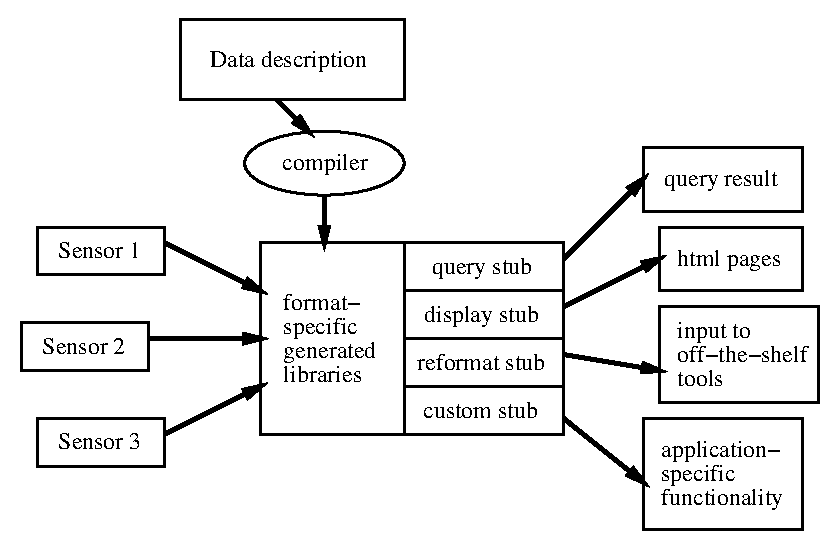
\psfig{file=arch_idraw_edit.ps,height=2.5in}}
\end{center}
\caption{\label{fig:arch} Architecture of Data-centric Monitor Generator.
}
\end{figure}

Together, the PI, David Walker (Princeton), Co-PI Vivek Pai
(Princeton) and Senior Personnel Kathleen Fisher (AT\&T Research) are
uniquely qualified to carry out this research as they bring the
necessary combination of skills in language design, compilers,
distributed systems, large-scale data processing, and practical system
monitoring as well as both academic and industrial perspectives to the
task.  In addition, they have already built a partial prototype system
(called PADS) to investigate the feasibility of the proposed ideas.
The prototype includes the preliminary design of a high-level, declarative
language for describing ad hoc data formats and a compiler capable of
generating parsing, printing, and reformatting libraries.

In the follow section, we will explain 
the architecture of a data-centric monitor generation system
and our prototype language design in more detail.  
Next, we will explain more of the specifics concerning
the generated tool suite for system monitoring.
In Section~\ref{ssec:features}, we will highlight some of the most
important language design challenges we face and
in Section~\ref{ssec:semantics}, we will propose a
formal system analysis to identify implementation errors
and improve system reliability.
In Section~\ref{ssec:impact}, we will explain how our research
on automatic generation of data processing tools
will make a broad impact on data processing that must be done
in disciplines well outside the bounds of
traditional computer science ranging from microbiology to physics to
economics.  We will also explain our education plan.

\subsection{A Data-Centric Monitor Generation System}

\paragraph*{Basic Architecture}
Figure~\ref{fig:arch} presents the architecture of our proposed
system.  At the top of the picture is the declarative description of all
data that will be used by the monitoring system.  It is here that
programmers encode all their knowledge about their data sources,
including the physical layout of data, its semantic properties
(including constraints on data fields and expected relations
with other fields) so deviations can be flagged as errors, 
its location, access protocol, when the data
will be ready for fetching and how often, etc.

In exchange for the programmer's work in describing their
data sources, the compiler system will generate
a robust and efficient library of {\em format-specific routines} (the center
square in the picture).
The core format-specific 
library includes parser, printer, error detection and data traversal
routines.  The core libraries will also be responsible for controlling
access to and aggregation of any data distributed across wide area
networks and archiving local data along with its description.  

Since these core libraries are compiler-generated from a
high-level data specification, they have many advantages over
hand-written code.  First, the generated code checks
all possible error cases: system errors related to the input file,
buffer, socket, or remote data provider; 
syntax errors related to deviations in the physical
format; and semantic errors in which the data violates user
constraints.  Because these checks appear only in generated code, they
do not clutter the high-level declarative description of the data
source.  Moreover, since tools are generated
automatically by a compiler rather than written by hand, 
they are far more likely to be robust
and far less likely to have dangerous vulnerabilities such as
buffer overflows.  Moreover, as formats change and are updated,
one can make a small change in the high-level description
and the compiler takes care of the rest.  It is extremely unlikely
new vulnerabilities or buffer overflows will be added to the code
base over time as formats change.  Finally, all routines will
be highly optimized for processing the massive
data sets one sees in practice.

In addition to the compiler, which generates the core, format-specific
libraries, the system includes a number of {\em format-independent stubs}
that make use of the generated libraries and implement higher-level
functionality.  Each of these stubs are programmed once, independent
of any format.  In order to implement format-specific behavior, they
are linked with the core libraries, which will be carefully designed to
satisfy a generic, format-independent interface.  Examples of
format-independent tools include a generic query engine that
allows users to extract information from the data, 
a visualization tool that produces
web page summaries of data statistics or a reformatter to convert data
to a new format required by an off-the-shelf tool.  In addition,
a programmer may simply use the generated format-specific libraries directly 
within their own application program, custom built for some unique task. 
Of course whenever a programmer builds a new tool for their application, 
they may do so using the format-independent interface to the generated
libraries.  If they do so, their new tool may be reused by others
who have different data, but require a similar functionality.

At this point, the astute reader may ask why not simply generate
exactly one tool -- a translator that maps the ad hoc data into
XML, a standard format with hundreds of available tools and
rich programming support in all modern, widely used languages.
The problem with such an architecture is that ad hoc formats
are usually quite compact and exploding them into XML representations
can easily result in a space blowup of 8-10 times and an increase
in processing overhead.  Consequently, tiny
sensors in a sensor network cannot afford the expense (processor,
network bandwidth, battery life) of managing
XML data.  More generally, when the data sets get large, and we 
have seen they do in monitoring systems, 
ranging from 100s of MB/week to 100GB/day,
the extra overhead of a 10 times blowup is simply unaffordable.
While compression can reduce this impact, the decompression overheads
of most modern compressors can overwhelm the data processing overhead
of the underlying data.
In an environment where the data is being used and updated
by more than just the monitoring systems, maintaining a parallel
representation in XML is even more painful and impractical.

\paragraph*{The Prototype Description Language}
To understand further how the \pads{} will be used,
let us look at an example of a simple ad hoc data source:
a tiny fragment of data in the Common Log Format (CLF) that web
servers use to log client requests~\cite{wpp}.  
This ASCII format consists of a sequence of
records, each of which has seven fields: the host name or IP address
of the client making the request, the account associated with the
request on the client side, the name the user provided for
authentication, the time of the request, the actual request, the
\textsc{http} response code, and the number of bytes returned as a
result of the request.  The actual request has three parts: the
request method (\eg, \texttt{GET}, \texttt{PUT}), the requested
\textsc{uri}, and the protocol version.  In addition, the second and
third fields are often recorded only as a '-' character to indicate
the server did not record the actual data.  \figref{figure:clf-records}
shows a couple of typical records.



\begin{figure*}
\begin{footnotesize}
%\begin{center}
\begin{verbatim}
207.136.97.49 - - [15/Oct/1997:18:46:51 -0700] "GET /tk/p.txt HTTP/1.0" 200 30
234.200.68.71 - - [15/Oct/1997:18:53:33 -0700] "GET /tr/img/gift.gif HTTP/1.0" 200 409
240.142.174.15 - - [15/Oct/1997:18:39:25 -0700] "GET /tr/img/wool.gif HTTP/1.0" 404 178
188.168.121.58 - - [16/Oct/1997:12:59:35 -0700] "GET / HTTP/1.0" 200 3082
tj62.aol.com - - [16/Oct/1997:14:32:22 -0700] "POST /spt/dd@grp.org/cfm HTTP/1.0" 200 941
214.201.210.19 ekf - [17/Oct/1997:10:08:23 -0700] "GET /img/new.gif HTTP/1.0" 304 -
\end{verbatim}
\caption{Tiny example of Common Log Format records. }
\label{figure:clf-records}
%\end{center}
\end{footnotesize}
\end{figure*}

With this example, we can examine how to use the prototype 
\pads{} language to describe 
the {\em physical layout} and 
{\em semantic properties} of our ad hoc data source. 
The language provides a type-based model:
basic types describe atomic data such as integers, characters, 
strings, dates, urls, \etc, while
structured types describe compound data built from simpler pieces.

In a bit more detail,
the \pads{} prototype provides a collection of broadly useful base
types.  Examples include 8-bit unsigned integers (\cd{Puint8}), 32-bit
integers (\cd{Pint32}), dates (\cd{Pdate}), strings (\cd{Pstring}),
and IP addresses (\cd{Pip}).  Semantic conditions for such base types
include checking that the resulting number fits in the indicated
space, \ie, 16-bits for \cd{Pint16}.  By themselves, these base types
do not provide sufficient information to allow parsing because they do
not specify how the data is coded, \ie{}, in ASCII, EBCDIC, or binary.
To resolve this ambiguity, \pads{} uses the \textit{ambient} coding,
which the programmer can set.  By default, \pads{} uses ASCII.  
% To
% specify a particular coding, the description writer can select base
% types which indicate the coding to use.  Examples of such types
% include ASCII 32-bit integers (\cd{Pa_int32}), binary bytes
% (\cd{Pb_int8}), and EBCDIC characters (\cd{Pe_char}).  In addition to
% these types, users can define their own base types to specify more
% specialized forms of atomic data.

To describe more complex data, the prototype provides a collection of
structured types loosely based on \C{}'s type structure.  In
particular, the prototype has \kw{Pstruct}s, \kw{Punion}s, and \kw{Parray}s
to describe record-like structures, alternatives, and sequences,
respectively.  \kw{Penum}s describe a fixed collection of literals,
while \kw{Popt}s provide convenient syntax for optional data.  Each of
these types can have an associated predicate that indicates whether a
value calculated from the physical specification is indeed a legal
value for the type.  For example, a predicate might require that two
fields of a \kw{Pstruct} are related or that the elements of a
sequence are in increasing order.  Programmers can specify such
predicates using \pads{} expressions and functions, written using a
\C{}-like syntax.  Finally, \pads{} \kw{Ptypedef}s can be used to
define new types that add further constraints to existing types.

\pads{} types can be parameterized by values.  This mechanism serves
both to reduce the number of base types and to permit the format and
properties of later portions of the data to depend upon earlier
portions.  For example, the base type \cd{Puint_FW(:x:)} specifies
an unsigned integer physically represented by exactly \cd{x}
characters, where \cd{x} is a value that has been read earlier in the
parse.  The type \cd{Pstring(:SPACE:)} describes a string
terminated by a space (when \texttt{SPACE} is defined to be \texttt{' '}).  
Parameters can be used with compound types like arrays and unions to
specify the size of an array or which branch of a union should be
taken.  This parameterization is what makes PADS a {\em dependently-typed}
language and substantially different from languages based on
context-free grammars or regular expressions.

\figref{figure:clf} gives a \pads{} description for the Common Log Format
data.  
We will use this example to illustrate some of the basic
features of the current \pads{} language.  
In \pads{} descriptions, types are declared before they are used, 
so the type that describes the totality of the data source appears 
at the bottom of the description.  
In this case,
the type \texttt{clf\_t}  describes the entirety of the
CLF data source (the \texttt{Psource} type qualifier indicates
this fact explicitly).  

\kw{Pstruct}s describe fixed sequences of data with unrelated types.
In the CLF description, the type declaration for
\cd{version_t} illustrates a simple \kw{Pstruct}. It starts with a 
string literal that matches the constant \cd{HTTP/} in the data source.  It 
then has two unsigned integers recording the major and minor version numbers
separated by the literal character \kw{'.'}.  \pads{} supports character, string,
and regular expression literals, which are interpreted with the ambient character 
encoding. The type \cd{request_t} 
similarly describes the request portion of a CLF record.  In addition
to physical format information, this \kw{Pstruct} includes a semantic constraint
on the \cd{version} field.  Specifically, it requires that obsolete methods
\cd{LINK} and \cd{UNLINK} occur only under HTTP/1.1.  This constraint illustrates
the use of predicate functions and the fact 
that earlier fields are in scope during the processing of later fields, as the 
constraint
refers to both the \cd{meth} and \cd{version} fields in the \kw{Pstruct}.

\kw{Punion}s describe variation in the data format.  For example, the
\cd{client_t} type in the CLF description indicates that the first
field in a CLF record can be either an IP address or a hostname.
During parsing, the branches of a \kw{Punion} are tried in order; the
first branch that parses without error is taken.  The \cd{auth_id_t}
type illustrates the use of a constraint: the branch \cd{unauthorized}
is chosen only if the parsed character is a dash.  \pads{} also
supports a \textit{switched} union that uses a selection expression to
determine the branch to parse.  Typically, this expression depends
upon already-parsed portions of the data source.

\pads{} provides \kw{Parray}s to describe varying-length sequences of
data all with the same type.  The \cd{clf_t} declaration  uses a
\kw{Parray} to indicate that a CLF file is a sequence of \cd{entry\_t}
records.  This particular array terminates when the data source is
exhausted. In general, \pads{} provides a rich
collection of array-termination conditions: reaching a maximum size,
finding a terminating literal (including end-of-record), or satisfying a
user-supplied predicate over the already-parsed portion of the \kw{Parray}. 
\pads{} also has convenient syntax for 
specifying separators that appear between elements of an array and
declaring inter-element constraints including sorting.

The
\kw{Penum} type \cd{method_t} describes a collection of data literals.
During parsing, \pads{} interprets these constants using the ambient
character encoding.  The \kw{Ptypedef} \cd{response_t} describes
possible server response codes in CLF data by adding the constraint
that the three-digit integer must be between 100 and 600.

Finally, the \kw{Precord} annotations deserve comment. It
indicates that the annotated type constitutes a record.  
The notion of a record varies depending upon the data encoding.  
ASCII data typically uses new-line characters to delimit 
records, binary sources tend to have fixed-width records, while 
COBOL sources usually store the length of each record before the actual data.
\pads{} supports each of these encodings of records and allows users to define
their own encodings.  By default, \pads{} assumes records are new-line terminated.
Before parsing, however, the user can direct \pads{} to use a different record
definition.
\texttt{Precords} have error-recovery semantics -- if errors 
in the data cause the parser to become seriously confused,
it will attempt to recover to a record boundary.
In practice, we have found this to be a very robust recovery mechanism
for ad hoc data.  

\begin{figure}
\begin{small}
\begin{code}
\kw{Punion} client\_t \{
  Pip       ip;      /- 135.207.23.32
  Phostname host;    /- www.research.att.com
\};
\mbox{}
\kw{Punion} auth\_id\_t \{
  Pchar unauthorized : unauthorized == '-';
  Pstring(:' ':) id;
\};
\mbox{}
\kw{Pstruct} version\_t \{
  "HTTP/";
  Puint8 major; '.';
  Puint8 minor;
\};
\mbox{}
\kw{Penum} method\_t \{
    GET,    PUT,  POST,  HEAD,
    DELETE, LINK, UNLINK
\};
\mbox{}
bool chkVersion(version\_t v, method\_t m) \{
  \kw{if} ((v.major == 1) && (v.minor == 1)) \kw{return} true;
  \kw{if} ((m == LINK) || (m == UNLINK)) \kw{return} false;
  \kw{return} true;
\};
\mbox{}
\kw{Pstruct} request\_t \{
  '\\"';   method\_t       meth;
  ' ';    Pstring(:' ':) req\_uri;
  ' ';    version\_t      version :
                  chkVersion(version, meth);
  '\\"';
\};
\mbox{}
\kw{Ptypedef} Puint16\_FW(:3:) response\_t :
         response\_t x => \{ 100 <= x && x < 600\};
\mbox{}
\kw{Precord} \kw{Pstruct} entry\_t \{
         client\_t       client;
   ' ';  auth\_id\_t      remoteID;
   ' ';  auth\_id\_t      auth;
   " ["; Pdate(:']':)   date;
   "] "; request\_t      request;
   ' ';  response\_t     response;
   ' ';  Puint32        length;
\};
\mbox{}
\kw{Psource} \kw{Parray} clf\_t \{
  entry\_t [];
\}
\end{code}
\end{small}
\caption{\pads{} description for Web Log data.}
\label{figure:clf}
\end{figure}

\subsection{Monitoring Framework}
\begin{figure*}[t]
\begin{center}
\centerline{\psfig{file=codeen_screen2.ps,width=5in}}
\end{center}
\caption{\label{fig_codeenmon}Screenshot of the CoDeeN monitoring
system, which is the model for our PADS-based system. Rows are
PlanetLab nodes, and most columns contain two data values, with the
column headings indicating the metrics being displayed. The bottom of
the window shows a 2-day history of any cell value. Other windows can
show histories on all nodes for a given metric, or histories of all
metrics for a is agiven node.}
\end{figure*}

To harness the power of PADS and make it easy to use for a variety of
system monitoring tasks, we will implement a generic monitoring
framework capable of scaling from monitoring single feeds at a single
location to monitoring data on thousands of machines in distributed
environments. This framework will consist of the following components:

\begin{enumerate}

\item {\bf Fetch} -- grab the data from one or more sources, in parallel if
needed, and perform whatever aggregation is necessary to begin parsing
the data. While this step may be application-specific, many
applications will use either TCP or UDP combined with a
request/response mechanism. By providing some example code for common
formats, such as HTTP/HTTPS, FTP/SFTP, SCP, SNMP, etc., we can reduce
or eliminate this portion of the ``buy-in'' cost for using our system.
While basic parameterization support will be included, this portion
will obviously be extensible, so that developers can customize it if
needed.

\item {\bf Display} -- once we have the raw data for one or more systems, we
can use the PADS specifications to drive extraction and formatting of
data for display. We will use HTML tables so that the data can be
viewed and manipulated interactively in Web browsers, but will also
support other export formats, such as plain text, CSV (comma-separated
values), tab-delimited format, and, where appropriate, XML
output. Using tables, we can devote one or more rows for each sensor,
machine, or instance, and show multiple data items as columns. In
cases where aggregate representations are appropriate, such as showing
sub-clusters, or multiple machines at a site, we can also show
composite information to summarize more information in the available
screen real estate. Since PADS can also automatically maintain
statistical information about the data it gathers, cell values can be
color-coded automatically, if no additional input is provided by the
developers.

\item {\bf Query} -- using the type information from the PADS description,
provide a mechanism where rows can be selected from the table based on
their contents. Users would be able to provide logical and arithmetic
expressions that could be evaluated using the per-row data, with the
selected rows being shown in the table format, or outputted to one of
the other formats mentioned above. This kind of support can be used to
easily identify sensors/machines behaving strangely, which need some
attention, or have situations of interest. For example, in a Grid
environment, when deploying a new experiment, it may be useful to
select the nodes with lower-than-average utilization.

\item {\bf Archive} -- the data fetched from the machines can be archived
along the with the description to process it. In this way, the data is
self-documenting, and can be accessed in the future using the same
tools as current data. The same support for viewing, querying, etc.,
can be applied to older data, allowing users to easily explore
behaviors over time. Given a reasonably robust description of the data
along with statistical information generated by PADS, it should also
be possible to optimize the on-disk format such that heavily-accessed
data is processed and cached in a post-processed, indexed form, even
if all of the data is stored in a raw format. This optimization can be
transparent to the developer and the users of the tools.

\end{enumerate}

What makes these tasks especially attractive in our context is that
they can be almost entirely automated given a well-formed data
description, making an interactive monitoring tool almost free, given
that the developer provides only slightly more information than is
necessary for parsing. Some of the extra information is entirely
presentational, such as the names used for displaying column headings
on data fields.

To get a sense of how this monitoring system can work, a screenshot of
the custom-built monitor for the CoDeeN content-distribution network
is shown in Figure~\ref{fig_codeenmon}. The entire process was
time-consuming and manual -- the display format and headings for each
row was manually specified, as was the sorting logic. The display
logic for each line was also manually written, to hide irrelevant
fields when nodes are dead or unreachable. Despite the fact that it
was developed for a specific project, it was widely used as a
general-purpose monitoring system for PlanetLab itself. Our proposal
will make generating such systems trivial, and will exploit
optimization opportunities that are time-consuming in
manually-generated systems. More importantly, as the data format
evolves, not only will the monitoring system automatically adapt, but
the archived data will still be available to the monitor, without
requiring multiple versions of the monitoring code for different points
in time.

\subsection{Automatic Format Inference}
\label{ssec:format-inference}

When a network problem, compromised machine or malfunctioning application
has been discovered, tracing the problem or attack to
prevent a recurrence is imperative.  This forensic analysis involves
human-guided study of multiple data sources such as log files and
other audit trails.  These data sources are great stores of
information, but they come in many varied and complex forms. They can
contain errors, either unintentional or malicious, and they can be
very, very large.  

To perform forensic analysis, analysts need to quickly understand a
variety of data sources and to ask specific questions about their
contents.  The variety, volume, and complexity of the data mean that
analysts need computational tools to support their analyses and to aid
in information extraction.  However, since every system is different
and the variety of data is so extensive, it is impossible to build
proactively all the specific tools one might need.

In the case of an attack, network forensic analysis should be done in
real-time, perhaps even while an attack is still underway. Not only
does this timeliness increase the chance of discovering the attacker
directly, it also provides the opportunity of identifying and
isolating compromised machines so that the attack cannot spread
further.  Of course, even in the case where an attack or problem is not
deemed urgent, a system adminstrator's time is always valuable --
improvements in administrator efficiency will be translated into 
improvements in their employer's bottom line.

Thus forensic analysts face a twofold problem: (1) they must be able
to ask questions of a wide array of data sources, impossible to
predict in advance, and (2) they must do so highly efficiently.  If
analysts faced only problem (1), they might take their time building
custom tools to query each individual data source from scratch, 
a task that might involve parsing, query support, and visualization 
components.  If analysts faced only problem (2) for a single data source 
known well in advance, they might take the initiative to develop a 
single, standard tool.  Our challenge is to solve both (1) and (2) 
simultaneously: to provide a platform for rapid generation of 
parsing, querying and visualization components for new and evolving
application data sources.

Although PADS descriptions can make managing ad hoc data much easier,
the problem of producing the description in the first place
remains. Writing such descriptions can be tedious and time consuming,
often requiring iteration. First, analysts write a description of as
much of the data as they understand. From this description, they
generate and run analysis tools to find any unknown parts of the
data. They then study those parts and refine the description
accordingly. They repeat this process until all the data either
conforms to the description or constitutes an error in the data rather
than an error in the description.  While the web server log we displayed
earlier may seem easy enough to describe by hand, it is amongst the
simplest examples that we could choose -- application logs may be much
more involved, requiring two-, three- or five-fold more complex descriptions.  
Moreover, the complexity of the situation grows tremendously in a realistic
setting where one must deal with logs of huge size (millions of lines long)
or large archives of logs of many different kinds. 
Having a tool to help produce such descriptions and to generate
data transformation and analysis tools automatically would speed up
forensic analysis and investigation efforts enormously.

\subsubsection*{Format Inference and Tool Generation Architecture}

\begin{figure}
\begin{center}
\centerline{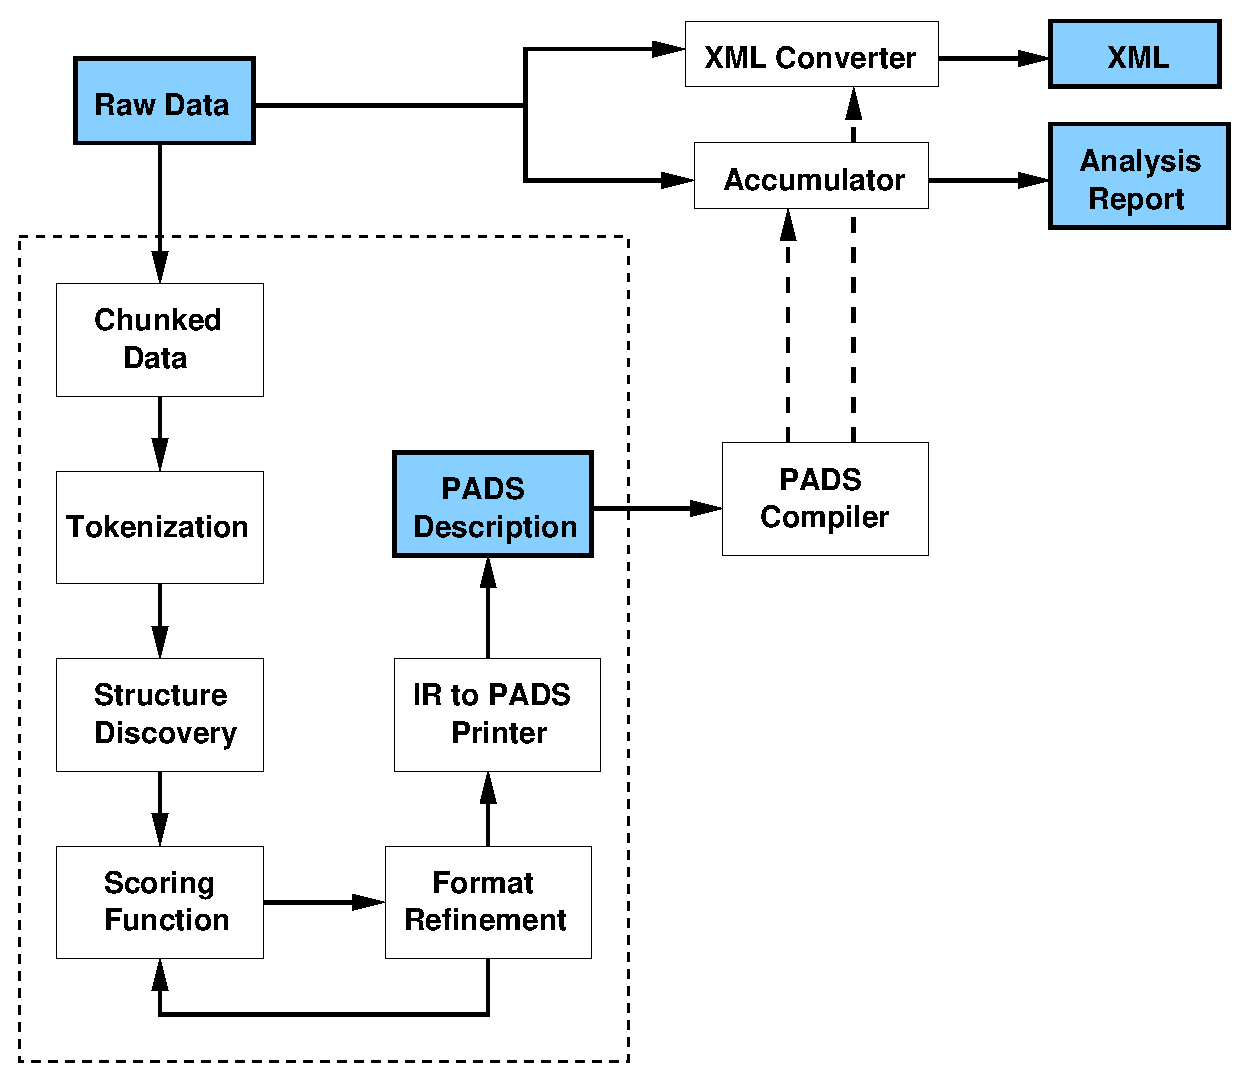
\psfig{file=format-inference-engine.eps,height=2.5in}}
\end{center}
\caption{Modular Architecture of a Format Inference and Tool Generation Engine}
\label{fig:format-inference-engine}
\end{figure}

In preparation for this proposal, we have begun to build a tool for
automatic format inference and data analysis tool generation.  In the
course of building this prototype we have defined a promising, modular 
architecture for solving the problem and performed some preliminary
experiments.  Our experiments have revealed the fact that our proposal
is indeed feasible yet many important challenges must be overcome
to turn our prototype into a robust, precise and viable system.

The overall architecture for the system is presented in
Figure~\ref{fig:format-inference-engine}.  As the diagram shows, the
system takes raw data (sets of systems or application logs) as an
input, pushes the raw data through the inference engine and generates
a \pads{} description.  This description is then automatically fed
through the current \pads{} compiler to produce several simple
data-processing tools including a tool that will read in the data and
translate it to \xml{} as well as a tool (listed in the diagram
as ``the accumulator'')
that will read in the data and output a simple statistical overview
of the data including the distribution of values in each data field and
the number of errors that it finds.

The heart of the system is a highly modular, multi-phase inference 
engine.  We have already begun work on each phase, but also have
many important research questions to answer about each part.
These phases include:

\begin{itemize}
\item {\bf Chunking:}  The first step in the inference process
is to break data into pieces, with the goal that each piece will have
a similar repetitive structure.  Currently, a user can
specify by hand that the data is either chunked line-by-line or file-by-file.
In the future we hope to develop techniques to handle several other
chunking strategies including paragraph-by-paragraph chunking or
directory-by-directory chunking of data sets.  We will develop heuristics
to guess the correct chunking structure when it is unspecified.

\item {\bf Tokenization:}  
The contents of every chunk of data must be divided up
into {\em tokens} such as numbers, words, punctuation, dates, times, 
ip addresses, phone numbers, etc.  Our current prototype includes built-in
support for a small number of basic tokens.  Our experiments indicate
effective tokenization is an extremely important element of the design, yet
astonishingly hard to achieve due ambiguities that arise in token definitions.
In particular, the {\em local} tokenization techniques we are currently using
seem insufficient for disamiguation in general and we are eager to investigate 
techniques that use more {\em global} information to achieve more precise
and useable tokenization.

\item {\bf Structure Discovery:}
After tokenization, the structure discovery phase produces a
candidate format for the data being analyzed.  This candidate is
produced through a recursive divide-and-conquer algorithm that uses
various heuristics to split the data into pieces, analyze the subpieces,
generate formats for subpieces and then combine generated formats to
create an overall description.  This divide-and-conquer algorithm
works well in many cases but occasionally fails, producing \pads{} 
descriptions that do not parse all of the data in the test set.
The reason for this failure is that not all \pads{} features (which
include features from context-free grammars as well as a certain kind
of {\em context-sensitive} grammar) will 
{\em compose} properly with one another.\footnote{Technically, we require
that if $D_1$ and $D_2$ are \pads{} descriptions, then the language of their
concatenation $L(D_1 . D_2)$ must be equivalent to the concatenation
of their languages $L(D_1) . L(D_2)$ and likewise for union and Kleene
closure.  \pads{}, which, for performance reasons, and to handle important
{\em non-context free} features such as dependencies and back references, 
is defined similarly
to the PEGS family of grammars does not have this critical property, 
which is the norm for context-free grammars.}  Hence, in order to overcome
this central problem and develop a robust inference engine, we must
investigate how to redesign several of the core elements of 
the \pads{} language, an interesting theoretical and implementation
challenge.

\item {\bf Scoring Function and Format Rewriting:}
The format generated by the structure discovery is only a rough ``guess''
at the structure of a format.  It is often unnecessarily complicated
in some places and too limited in others.  In order to improve the 
quality of the guess, we score the format and then search for ways
to optimize it using a collection of format rewriting rules.  The
score is based upon the information-theoretic principles embodied in
the Minimum Description Length Principle (MDL)~\cite{mdl}.  In our
experience to date, this format rewriting is somewhat effective --
it reduces the score of the formats initially produced substantially.
However, to the human eye, much improvement can still be made.  We must
investigate the sources of the problems, develop new rewriting rules
and refine the scoring function which guides which rules to apply and
when. 
\end{itemize}

In addition to studying, evaluating, and improving each of the phases
of the inference engine mentioned above, we will engage in two additional
tasks with regards to this element of the grant:

\begin{itemize}
\item {\bf Scaling to large data sets:}
\item {\bf Wholistic repository inference:}
\end{itemize}

\paragraph*{Summary of Format Inference:}  
We have developed a prototype
format inference engine for system log files.  This prototype demonstrates
our ability and the viability of our approach.  However, all phases of
our prototype engine (chunking, tokenization, structure discovery,
scoring and rewriting) must be improved in order to deliver a reliable and
effective automatic tool generation engine.  Moreover, we must develop
completely new algorithms in order to scale our current system up to 
be able to handle application log files of realistic size and complexity.
Finally, we must develop new techniques to extend the scope of our engine
so that it can analyze and uncover the structure
of entire repositories full of log files.

%\subsection{Towards a Universal Data Description System}
%\label{ssec:features}
%
In this section, we discuss the principal limitations of the \pads{}\ 
infrastructure we have built to date and explain extensions
necessary to build data-centric system monitors. 

\paragraph*{Multi-source Monitoring}
The current \pads{} specification language can only describe
the contents of a single, fixed data source.  In order to 
generate monitoring infrastructure for
wide area distributed systems such as the Grid, which 
may contain hundreds or thousands of nodes, each 
potentially with several different sensors producing
new data at a rapid rate, we must augment \pads{}
so that it may specify a collection of data sources
both local to a single machine and distributed across a wide area network.
In addition, it will be necessary to describe the {\em temporal}
aspects of data collection -- will data be pulled to a central
processor next Tuesday (only), once per day, once every five minutes
or triggered by user, network or other conditions?
In order to support multi-source monitoring, we will augment PADS
with the following features and implementation support.

% For example, in order to monitor the health of PlanetLab, a
% distributed network of several hundred machines spread across the
% world, the CoMon monitoring system~\cite{comon} attempts to drag a
% small data file from each of the machines to a centralized repository
% once every five minutes.  In the centralized repository, the data is
% split into two new formats, each designed to accumulate information
% about a certain aspect of the system.  In all, CoMon produces
% approximately 22,000 files/day.    We
% propose to extend our specification language to enable automatic
% generation of tools that process multiple data sources, either on one
% local machine or distributed across a wide area network.  Doing so
% will require investigation of the following features.

\begin{enumerate}
\item {\bf Multi-source Specifications}  
We propose to extend the PADS specification language with a new
first-class type constructor, \texttt{Pget\{T;e\}}.  Here \texttt{e}
specifies a protocol for locating and accessing a data source, and
\texttt{T} is a PADS type specifying the structure of its contents.
The specification language for protocols should be completely flexible
so it can handle the largest possible collection of applications.  For
instance, CoMon accesses data via telnet and authentication; other
data is available over the web through FTP and HTTP.  
Though the construct \texttt{Pget \{T;e\}}, 
is simple (an explicit design choice) we believe that 
when it interacts with the rest of the PADS
specification language it will provide powerful access possibilities.
In particular, due to the dependency already present in PADS, it will
be possible to read a local file containing information
concerning when, where and how to acquire further data and
then use \texttt{Pget} recursively to implement distributed data collection. 
For instance, to implement a CoMon-like monitoring
service, a local machine might contain a list of all current
PlanetLab nodes.  A PADS specification might read that list and use
the information processed to acquire information from all machines on
the list.  Such a data-driven architecture allows dynamic changes
to network structure while leaving the monitoring infrastructure unchanged.

\item {\bf Temporal Specifications}
In order to support applications that monitor repeated, ongoing phenomena, we
will need to add temporal specifications to PADS.  These
temporal specifications might indicate periodic arrival of new data
(once every five minutes), arrival of data at some specific time in
the future (next Tuesday) or upon receiving an explicit signal from
some external source such as a user.  
As is the case with our spatial specification
\texttt{Pget}, we will strive for a design that combines simplicity
with generality.  We anticipate adding a second symmetric operator to PADS,
\texttt{Ptime} that specifies when to take action, and a 
domain-specific temporal language for specifying times.  However, 
it will take substantial research
to work out the details of a sufficiently flexible, yet concise
and easy-to-understand temporal specification language. 
We plan to investigate all corners of the design space.

\item {\bf Concurrent Execution}  
PADS is currently a single-threaded application.  However,
to support access to many sources, possibly distributed
across a wide area, it will be necessary to process multiple
repositories concurrently.  As data from each new source is requested
through the \texttt{Pget} command, we plan on launching a new thread
to read the source.  However, the dependency in PADS may
require synchronization between threads, making implementation
of parallel processing nontrivial.  More research is required to
understand the optimal implementation strategy.  However, the fact that
PADS is a pure, declarative language should simplify dependency
analysis greatly and improve opportunities to hide latency through
concurrency.


% BS alert!!

\item {\bf Modular Specifications}
As specifications begin to get larger and encompass multiple different
data repositories, possibly with different data formats, standard
software engineering practice suggests introduction of features to
enable modular development of specifications and to allow multiple
programmers to collaborate on specifications.  The first necessary
addition to PADS along these lines is a namespace mechanism to allow
programmers to control their type names in a disciplined fashion.  A
second extension we will explore is introduction of more general
interfaces that allow programmers to make type definitions abstract.
This feature should make it easier to evolve large specifications as
monitoring requirements change.

\end{enumerate}


\paragraph*{Data Transformation, Compression, Encryption and Error-correction}
The data used by monitoring systems may require simple transformations 
of various kinds
immediately before parsing or after parsing and before
passing data to downstream processors, query engines or 
visualization tools.  Before archiving data,
inverse transformations may have to be applied.  
Examples of pre-parsing routines include decryption for
security-sensitive data and decompression for high-volume data.  
The natural inverses for printing and archiving 
are encryption and compression.
After parsing, many data sources require, or at least benefit from,
a variety of simple data transformations.  For example,
sometimes poorly-designed
ad hoc data will have multiple different representations
of the same concept -- dates in different formats, several different strings
to represent ``no value'' etc.  Simple transforms can be used to convert
these representations into a canonical form that facilitates down-stream
processing.  As another example, many data sources have privacy-sensitive parts
that should be ``sanitized'' in some way or another, possibly by scrubbing or
filtering data fields before passing them to down-stream applications.
In October 2005, for instance, we asked the Princeton Computer Science
Department Technical Staff for access to web logs for some experiments
with \pads, but they refused until they had written scripts to
sanitize the data for us.  Medical data is another example of highly
privacy-sensitive data.
Lastly, almost all ad hoc data may contain errors, but sometimes there 
will be simple data-specific heuristics such as substitution of default values
or discarding of corrupted segments
that can be used to fix the most common problems.

It is currently impossible to code multi-stage processing and transformation
directly in PADS.  One solution
to this problem might be to let auxiliary passes through the data
remain outside the PADS system as prepasses or postpasses.  
Unfortunately, this solution is completely unsatisfactory for a
number of reasons.  First, doing so
will often leave us in a situation in which the \pads{} description 
is not a self-contained
definition of the data format in question.  Consequently some of the value
of \pads{} as documentation is lost.  
Second, programmers must do
more work themselves to produce PADS applications.  They cannot
simply run our automatic generators and receive a well-packaged 
query engine or statistical analyzer for the raw data.
Moreover, when coding transformation directly in C, the host language
for \pads{}, they must program at a much lower level of abstraction
than we might provide by supplying specialized domain-specific
transformers directly in \pads.
Since our goal is to maximize the productivity of scientists 
who use ad hoc data, ease-of-use is a key constraint.
Finally, some data formats and
tasks are not well-suited for implementation as a separate pre- or post-pass.
For example, some formats use non-uniform compression or encryption 
schemes~\cite{korn+:delta,korn+:data-format}.
Moreover, tasks such as data sanitization and error correction may be
data-dependent and directed by the structure of the data.  In other words,
they may involve just the sort of data analysis that PADS was built for
and should be integrated directly into the specification mechanism.

To address these difficulties,
we plan to research mechanisms that facilitate multi-stage data processing 
directly in PADS.  Since any PADS description must be able to generate 
both data
input tools {\em and} data output tools, we currently believe that each
data processing stage, or layer, should be specified as a pair of
transformations.  For instance, if data is decompressed on the way in,
it must be compressed on the way out.  If a field of the data is ``sanitized''
or filtered on the way in, perhaps a default value of the correct form must
be written back out to preserve the syntactic structure of the data format.

To achieve this functionality, we will begin by considering a
transformation specification with the general form 
\texttt{Ptransform \{ i,o :  Tcon <-> Tabs \}}.
Here, {\tt Tcon} is the PADS type of the external or {\tt con}crete
representation and {\tt Tabs} is the PADS type of the internal or 
{\tt abs}tract representation.  The internal representation of the current
phase may in turn serve as the external representation for the next
phase of the transformation.  The functions {\tt i} and {\tt o} are
user-defined functions that transform data from {\tt Tcon} to 
{\tt Tabs} and vice versa.  For example, {\tt i} may implement
decompression and {\tt o} may implement compression.

We intend to add these transformations as first-class
descriptions/types to the system.  In other words, these
transformation may be nested inside or otherwise composed with any
other form of PADS description.  When so nested, the transformation
will only apply to the appropriate specific subcomponent of the
format.  Therefore, transformations will be useful for simple
subcomponent error correction or representation casting as well as
full data source transformations such as decompression.  In addition,
transformations with compatible types will be composable.  For
example, if a data format is compressed and potentially contains
errors, a decompression transform may be composed with an
error-correction transform.

The meat of certain transformations such as compression and encryption
are probably best written as ordinary program code that is
subsequently included in the PADS description.  However, for smaller
scale, local transformations, we will investigate adding domain-specific
programming support.  This support would allow programmers to write
transforms quickly at an easy-to-understand and high level
abstraction.  It would also ensure that the output transformations are
proper inverses of the inputs.  In particular, inspired by recent work
by Foster et al.~\cite{foster+:lens}, we will explore how to develop a
library of {\em combinators}, simple composable functions, that can be
combined in a myriad of ways to produce the transforms {\em and their
inverses} at the same time.  Foster et al. used such bi-directional transforms to
solve a synchronization problem on error-free tree-shaped data. 
While we will exploit some of their
ideas, our application and
context are different: we are parsing, transforming, querying, archiving
and presenting system monitoring data.
As we do so, we are specifically interested in uncovering,
representing and handling error-filled data.  One of the critical
challenges for us will be to design the combinators so that they deal
with \pads{} parse descriptors correctly
and conveniently.



%\subsection{Formalization and Semantic Analysis}
%\label{ssec:semantics}
%\documentclass[11pt]{article}

\usepackage{xspace,amsmath,math-cmds,
            math-envs,times,
            verbatim,multicol,proof,url}
\usepackage{code} 
\usepackage{epsfig}
\renewcommand{\bar}[1]{\overline #1}
\newcommand{\base}{{\tt Base}}
\newcommand{\sync}{{\tt Sync}}
\newcommand{\mystruct}{{\tt Struct}}
\newcommand{\myunion}{{\tt Union}}
\newcommand{\myarray}{{\tt Array}}
\newcommand{\D}{{\mathbb D}}
\newcommand{\cut}[1]{}
\newcommand{\reminder}[1]{{\it #1 }}
\newcommand{\edcom}[1]{\textbf{{#1}}}
\newcommand{\poplversion}[1]{#1}
\newcommand{\trversion}[1]{}

\newcommand{\appref}[1]{Appendix~\ref{#1}}
\newcommand{\secref}[1]{Section~\ref{#1}}
\newcommand{\tblref}[1]{Table~\ref{#1}}
\newcommand{\figref}[1]{Figure~\ref{#1}}
\newcommand{\listingref}[1]{Listing~\ref{#1}}
%\newcommand{\pref}[1]{{page~\pageref{#1}}}

\newcommand{\eg}{{\em e.g.}}
\newcommand{\cf}{{\em cf.}}
\newcommand{\ie}{{\em i.e.}}
\newcommand{\etal}{{\em et al}}
\newcommand{\etc}{{\em etc.\/}}
\newcommand{\naive}{na\"{\i}ve}
\newcommand{\role}{r\^{o}le}
\newcommand{\forte}{{fort\'{e}\/}}
\newcommand{\appr}{\~{}}

\newcommand{\bftt}[1]{{\ttfamily\bfseries{}#1}}
\newcommand{\kw}[1]{\bftt{#1}}
\newcommand{\pads}{\textsc{pads}}
\newcommand{\padsc}{\textsc{pads/c}}
\newcommand{\padx}{\textsc{padx}}
\newcommand{\ipads}{\textsc{ipads}}
\newcommand{\ir}{\textsc{IR}}
\newcommand{\padsl}{\textsc{padsl}}
\newcommand{\padsml}{\textsc{pads/ml}}
%\newcommand{\padsd}{\textsc{pads/d}}
\newcommand{\learnpads}{{\textsc{learnpads}}}
\newcommand{\padsd}{\textsc{Gloves}}
\newcommand{\blt}{\textsc{blt}}
\newcommand{\ddc}{\textsc{ddc}}
\newcommand{\ddl}{\textsc{ddl}}
\newcommand{\C}{\textsc{C}}
\newcommand{\perl}{\textsc{Perl}}
\newcommand{\ml}{\textsc{ml}}
\newcommand{\smlnj}{\textsc{sml/nj}}
\newcommand{\ocaml}{\textsc{OCaml}\xspace}
\newcommand{\haskell}{\textsc{haskell}\xspace}
\newcommand{\ocamlbig}{\textsc{OCAML}\xspace}
\newcommand{\java}{\textsc{java}}
\newcommand{\xml}{\textsc{xml}}
\newcommand{\html}{\textsc{html}}
\newcommand{\xpath}{\textsc{xpath}}
\newcommand{\xquery}{\textsc{xquery}}
\newcommand{\datascript}{\textsc{datascript}}
\newcommand{\packettypes}{\textsc{packettypes}}
\newcommand{\erlang}{\textsc{Erlang}}
\newcommand{\camlp}{\cd{Camlp4}}
\newcommand{\ocamlnet}{\cd{Ocamlnet} \cd{2}}

\newcommand{\totalcost}[2]{\textsc{Cost}(#1,#2)}
\newcommand{\costdescription}[1]{\textsc{CT}(#1)}
\newcommand{\normcostdescription}{\textsc{NCT}}
\newcommand{\costdata}[2]{\textsc{CD}(#2 \; | \; #1)}
\newcommand{\acostdata}[2]{\textsc{ACD}(#2 \; | \; #1)}
\newcommand{\adc}[2]{\textsc{CD'}(#2 \; | \; #1)}
\newcommand{\cardt}{\textsc{Card}}
\newcommand{\costvar}[1]{\textsc{CV}(#1)}
\newcommand{\costchar}[1]{\textsc{CA}(#1)}
\newcommand{\coststring}[1]{\textsc{CS}(#1)}
\newcommand{\costint}[1]{\textsc{CI}(#1)}
\newcommand{\costparam}[1]{\textsc{CP}(#1)}
\newcommand{\costconst}[1]{\textsc{CC}(#1)}

\newcommand{\dibbler}{Sirius}
\newcommand{\ningaui}{Altair}
\newcommand{\darkstar}{Regulus}

\newcommand{\vizGems}{Arrakis}

\newcommand{\comon}{CoMon\xspace}
\newcommand{\planetlab}{PlanetLab\xspace}
\newcommand{\monall}{Monall\xspace}
%% \newcommand{}{}


%% \newcommand{\IParray}[4]{{\tt Parray} \; #1 \; \[#2, #3, #4\]}

\newcommand{\figHeight}[4]{\begin{figure}[tb]
	\centerline{
	            \epsfig{file=#1,height=#4}}
	\caption{#2}
	\label{#3}
	\end{figure}}

\newcommand{\myalt}{\ensuremath{\; | \;}}
\newcommand{\normal}[1]{\ensuremath{\bar{#1}}}
\newcommand{\relativee}[2]{\ensuremath{{\cal R}(#1 \; || \; #2)}}
\newcommand{\srelativee}[2]{\ensuremath{{\cal S}(#1 \; || \; #2)}}
\newcommand{\addh}[2]{\ensuremath{#1 \oplus #2}}

\newcommand{\irstruct}[1]{{\tt struct}\{#1\}}
\newcommand{\irunion}[1]{{\tt union}\{#1\}}
\newcommand{\irenum}[1]{{\tt enum}\{#1\}}
\newcommand{\irarray}[1]{{\tt array}\{#1\}}
\newcommand{\irarrayFW}[2]{{\tt arrayFW}\{#1\}[#2]}
\newcommand{\irswitch}[2]{{\tt switch}(#1)\{#2\}}
\newcommand{\iroption}[1]{{\tt option}\{#1\}}
\newcommand{\setof}[1]{\lsem #1 \rsem}
\newcommand{\goto}{\Rightarrow}
\newcommand{\Pvoid}{{\tt Pvoid}}
\newcommand{\Pempty}{{\tt Pempty}}
\newcommand{\sskip}{\hspace*{5mm}}
\newcommand{\shrink}{\vspace*{-4mm}}

% Semantics
\newcommand{\setalt}{{\; | \;}}
\newcommand{\denote}[1]{\lsem #1 \rsem}
\newcommand{\lsem}{{[\![}}
\newcommand{\rsem}{{]\!]}}
\newcommand{\turn}{\vdash}
\newcommand{\meta}{m}
\newcommand{\nested}{n}
\newcommand{\mytime}[1]{#1.t}
\newcommand{\myds}[1]{#1.ds}
\newcommand{\myval}[1]{#1.nest}
\newcommand{\generatedloc}{\ensuremath{\mathtt{nowhere}}}
\newcommand{\environment}{E}
\newcommand{\universe}{U}
\newcommand{\selectOne}{\ensuremath{\mathsf{earliest}}}
% core feed semantics
\newcommand{\csemantics}[3]{{\cal C}\lsem #1 \rsem_{{#2} \, {#3}}}
% feed semantics
\newcommand{\semantics}[3]{{\cal F}\lsem #1 \rsem_{{#2} \, {#3}}}
% expression semantics
\newcommand{\esemantics}[2]{{\cal E}\lsem #1 \rsem_{{#2}}}
%\newcommand{\esemantics}[2]{#2(#1)}

% Host language types
\newcommand{\ty}{\ensuremath{\tau}}
\newcommand{\basety}{\ensuremath{b}}
\newcommand{\arrow}{\rightarrow}
\newcommand{\optionty}[1]{\ensuremath{#1 \; \mathsf{option}}}
\newcommand{\listty}[1]{\ensuremath{#1 \; \mathsf{list}}}
\newcommand{\setty}[1]{\ensuremath{#1 \; \mathsf{set}}}
\newcommand{\feedty}[1]{\ensuremath{#1 \; \mathsf{feed}}}
\newcommand{\corety}[1]{\ensuremath{#1 \; \mathsf{core}}}
\newcommand{\schedulety}{\ensuremath{\mathsf{sched}}}
\newcommand{\timety}{\ensuremath{\mathsf{time}}}
\newcommand{\locty}{\ensuremath{\mathsf{loc}}}
\newcommand{\boolty}{\ensuremath{\mathsf{bool}}}
\newcommand{\unitty}{\ensuremath{\mathsf{unit}}}
\newcommand{\stringty}{\ensuremath{\mathsf{string}}}
\newcommand{\metatype}[1]{\ensuremath{\mathsf{meta}(#1)}}
\newcommand{\nestedtype}[1]{\ensuremath{\mathsf{nest}(#1)}}
\newcommand{\dsty}{\ensuremath{\mathsf{ds}}}

\newcommand{\dom}{\ensuremath{\mathsf{dom}}}
\newcommand{\ueq}[3]{\ensuremath{#1 =_{#2} #3}}
\newcommand{\fsubset}[3]{\ensuremath{#1 \subseteq_{#2} #3}}
\newcommand{\feq}[3]{\ensuremath{#1 =_{#2} #3}}

% Expressions
\newcommand{\expression}{e}
\newcommand{\constant}{c}
\newcommand{\ds}{\ensuremath{ds}}
\newcommand{\boolf}{\ensuremath{\mathtt{false}}}
\newcommand{\boolt}{\ensuremath{\mathtt{true}}}
\newcommand{\loc}{\ensuremath{\ell}}
\newcommand{\feed}{\ensuremath{F}}
\newcommand{\corefeed}{\ensuremath{C}}
\newcommand{\generalvar}{\ensuremath{x}}
\newcommand{\feedvar}{\ensuremath{x}}
\newcommand{\itemvar}{\ensuremath{x}}
\newcommand{\data}{\ensuremath{v}}
\newcommand{\atime}{\ensuremath{t}}
\newcommand{\astring}{\ensuremath{w}}
\newcommand{\unit}{\ensuremath{()}}
\newcommand{\schedule}{\ensuremath{s}}
\newcommand{\parser}{\ensuremath{p}}
\newcommand{\none}{\ensuremath{\mathtt{None}}}
\newcommand{\some}[1]{\ensuremath{\mathtt{Some}\; #1}}
\newcommand{\inl}[1]{\ensuremath{\mathtt{inl}\; #1}}
\newcommand{\inr}[1]{\ensuremath{\mathtt{inr}\; #1}}
\newcommand{\casedata}[2]{{\tt switch}(#1)\{#2\}}
%\newcommand{\nillist}{\ensuremath{\mathtt{nil}}}
\newcommand{\nillist}{\ensuremath{[\,]}}
%\newcommand{\conslist}[2]{\ensuremath{\mathtt{cons} (#1,#2)}}
\newcommand{\conslist}[2]{\ensuremath{[#1,\ldots,#2]}}
\newcommand{\nilstream}{\ensuremath{\mathtt{done}}}
\newcommand{\consstream}[2]{\ensuremath{\mathtt{next} (#1,#2)}}


% Feeds
\newcommand{\comprehensionfeed}[3]{\ensuremath{\mathtt{\{|} #1 \; \mathtt{|}\; #2 \leftarrow #3 \mathtt{|\}}}}
\newcommand{\computed}[3]{\ensuremath{\mathtt{[} #1 \; \mathtt{|}\; #2 \in #3 \mathtt{]}}}
\newcommand{\letfeed}[3]{\ensuremath{\mathtt{let}\; #1 \; \mathtt{=}\; #2 \; \mathtt{in} \; #3}}
\newcommand{\allfeed}[5]{
  \ensuremath{
    \mathtt{all \{ format=} #1; 
    \mathtt{src=} #2;
    \mathtt{sched=} #3;
    \mathtt{pp=} #4;
    \mathtt{win=} #5;
  \mathtt{\}}}}
\newcommand{\existsfeed}[5]{
  \ensuremath{
    \mathtt{any \{ format=} #1; 
    \mathtt{src=} #2;
    \mathtt{sched=} #3;
    \mathtt{pp=} #4;
    \mathtt{win=} #5;
  \mathtt{\}}}}
\newcommand{\filterfeed}[2]{
  \ensuremath{
    \mathtt{filter} \; #1 \; \mathtt{with}\; #2}}
\newcommand{\remapfeed}[2]{
  \ensuremath{
    \mathtt{redirect} \; #1 \; \mathtt{with}\; #2}}
\newcommand{\ppfeed}[2]{
  \ensuremath{
    \mathtt{pp} \; #1 \; \mathtt{with}\; #2}}
\newcommand{\foreachupdate}[3]{
  \ensuremath{
    \mathtt{foreach{*}{*}}\; #1 \;
    \mathtt{in}\; #2 \;
    \mathtt{update}\; #3}}
\newcommand{\foreachcreate}[3]{
  \ensuremath{
    \mathtt{foreach*}\; #1 \;
    \mathtt{in}\; #2 \;
    \mathtt{create}\; #3}}
\newcommand{\remap}[2]{\ensuremath{\mathtt{redirect}\; #1 \; \mathtt{with} \; #2}}
\newcommand{\stutterfeed}[2]{\ensuremath{\mathtt{stutter}\; #1 \; \mathtt{on} \; #2}}
\newcommand{\refeed}[2]{\ensuremath{\mathtt{reschedule}\; #1 \; \mathtt{to} \; #2}}
\newcommand{\emptyfeed}{\ensuremath{\emptyset}}
\newcommand{\onefeed}[2]{\ensuremath{\mathtt{One}}(#1,#2)}
\newcommand{\sfeed}[1]{\ensuremath{\mathtt{SchedF}}(#1)}
\newcommand{\lfeed}[1]{\ensuremath{\mathtt{ListF}}(#1)}
\newcommand{\unionfeed}{\ensuremath{\cup}}
\newcommand{\sumfeed}{\ensuremath{+}}
\newcommand{\spairfeed}{\; \ensuremath{\mathtt{\&} \; }}
\newcommand{\allpairfeed}{\; \ensuremath{{*}{*}} \; }

\newcommand{\Time}{\ensuremath{\mathtt{Time}}}
\newcommand{\Set}{\ensuremath{\mathtt{Set}}}

% this is used for the translations equal
\newcommand{\transeq}{\stackrel{def}{=} }
\newcommand{\ai}{{\tt wl}}



% BNF
%\newcommand{\bnfalt}{\ |\ }

\begin{document}

\section{Preliminary Definitions}

\noindent
$s$: a character string \\
$s_1 s_2$: concatenation of strings $s_1$ and $s_2$\\
$s_1 - s_2$: prefix of $s_1$ that is not a substring of $s_2$ \\
$\D$: an annotated description \\
$e$: error code \\
$d$: (error code, string) pair\\
$\bar x$: a list of $x$ \\
$L(B)$: language accepted by $B$\\
$\oplus$: binary operators on two error codes\\
$l_1 @ l_2$: concatenation of two lists\\
$l[x'/x]$: substitution of $x'$ for $x$ in list $l$

\begin{eqnarray*}
e &::=& G \bnfalt F \bnfalt P ~~~ {\rm (Good,~ Fail~ or~ Partial)}\\
\D &::=& nil \bnfalt \base~ \bar{d} \bnfalt \sync~ \bar{d} \bnfalt \mystruct~ \bar{d}~  \bar{\D} \bnfalt 
\myunion~ \bar{d}~ \bar{\D} \bnfalt \myarray~ \bar{d}~ (\D, \D_s, \D_t)
\end{eqnarray*}

\begin{eqnarray*}
G \oplus G &=& G\\
G \oplus F &=& P\\
G \oplus P &=& P\\
F \oplus F &=& F\\
F \oplus P &=& P\\
P \oplus P &=& P
\end{eqnarray*}

\section{Operational Semantics}
Main judgement (consumption of string data):

\noindent
\[s,~ \D \leadsto s',~ \D',~ e'\]

\noindent
where $e'$ is the is the error code of the last data item in $\D'$.

\[
\infer[\rm{(Base-G)}]{s_1 s_2,~ \base~ \bar{d} \leadsto s_2,~ \base~ \bar{d}@[(G,~ s_1)],~ G}
{s_1 \in L(\base)} 
\]

\[
\infer[\rm{(Base-F)}]{s,~ \base~ \bar{d} \leadsto s,~ \base~ \bar{d} @ [(F,~ "")],~ F}
{{\rm prefix}(s) \cap L(\base) = \emptyset}
\]

\[
\infer[\rm{(Sync-G)}]{s_1 s_2,~ \sync~ \bar{d} \leadsto s_2,~ \sync~ \bar{d}@[(G,~ s_1)],~ G}
{s_1 \in L(\base)} 
\]

\[
\infer[\rm{(Sync-F)}]{s,~ \sync~ \bar{d} \leadsto s,~ \sync~ \bar{d} @ [(F,~ "")],~ F}
{{\rm substring}(s) \cap L(\sync) = \emptyset}
\]

\[
\infer[\rm{(Sync-P)}]{s_1 s_2 s_3,~ \sync~ \bar{d} \leadsto 
s_3,~ \sync~ \bar{d} @ [(P,~ s_1 s_2)],~ P}
{{\rm substring}(s_1) \cap L(\sync) = \emptyset  & s_2 \in L(\sync)}
\]

\[
\infer[\rm{(Struct)}]{s_1,~ \mystruct~ \bar{d}~ [\D_1, \ldots, \D_n] \leadsto 
s_{n+1},~ \mystruct~ \bar{d} @ [(e',~ s_1 - s_{n+1})]~ [\D_1', \ldots, \D_n'],~ e'}
{
\forall i \in [1,~ n]:~ s_i,~ \D_i \leadsto
s_{i+1},~ \D_i',~ e_i'~~~~~~~  e' = e_1' \oplus \ldots \oplus e_n'
}
\]

\[
\infer[\rm{(Union-G)}]
{
\begin{array}{c}
s,~ \myunion~ \bar{d}~ [\D_1, \ldots, \D_{m-1}, \D_m, \D_{m+1}, \ldots, \D_n] \leadsto \\
s_m',~ \myunion~ \bar{d} @ [(G, s - s_m')]~ , [\D_1, \ldots, \D_{m-1}, \D_m', \D_{m+1},\ldots, \D_n], G
\end{array}}
{
\begin{array}{c}
\forall i \in [1, m-1], 1 \le m \le n-1 :~ s, \D_i \leadsto s_i', \D_i', e_i' ~~~~ e_i' \in \{F,~ P\} \\
s,~ \D_m \leadsto s_m',~ \D_m', G\\
\end{array}
}
\]

\[
\infer[\rm{(Union-Last)}]
{
\begin{array}{c}
s,~ \myunion~ \bar{d}~ [\D_1, \ldots, \D_{n-1}, \D_n] \leadsto \\ 
s_n',~ \myunion~ \bar{d} @ [(e_n', s - s_n')]~ [\D_1, \ldots, \D_{n-1}, \D_n'], e_n'
\end{array}}
{
\begin{array}{c}
\forall i \in [1, n-1]:~ s_i, \D_i \leadsto s_i', \D_i', e_i' ~~~~ e_i' \in \{F,~ P\} \\
s,~ \D_n \leadsto s_n',~ \D_n', e_n'\\
\end{array}
}
\]

\[
\infer[\rm{(Array-1)}]{
\begin{array}{c}
s_1 \cdots s_{n+2},~  \myarray~ \bar{d}~ (\D_1,~ \D_{s,1},~ \D_t) \leadsto \\
s_{n+2},~ \myarray~ \bar{d} @ [(e_1 \oplus \ldots \oplus e_n, s_1 \cdots s_{n+1})]~ 
(\D_{n+1},~ \D_{s, n+1},~ \D_t'),~ e_1 \oplus \ldots \oplus e_n
\end{array}}
{
\begin{array}{c}
\forall i \in [1,~ n-1]: s_i \cdots s_{n+2},~ \mystruct~ nil~ [\D_i,~ \D_{s,i}] \leadsto \\
s_{i+1} \cdots s_{n+1},~ \mystruct~ [(e_i, s_i)] [\D_{i+1},~ \D_{s,i+1}],~ e_i ~~~~ e_i \in \{G,~ P\}\\ 
s_n s_{n+1} s_{n+2}, \D_n \leadsto s_{n+1} s_{n+2}, \D_{n+1}, e_n ~~~~ e_n  \in \{G,~ P\} \\
s_{n+1} s_{n+2}, \D_t \leadsto s_{n+2}, \D_t', G
\end{array}
}
\]

\[
\infer[\rm{(Array-2)}]{
\begin{array}{c}
s_1 \cdots s_n,~  \myarray~ \bar{d}~ (\D_1,~ \D_{s,1},~ \D_t) \leadsto \\
s_n,~ \myarray~ \bar{d} @ [(e_1 \oplus \ldots \oplus e_{n-1}, s_1 \cdots s_{n-1})]~ 
(\D_n,~ \D_{s, n},~ \D_t),~ e_1 \oplus \ldots \oplus e_{n-1}
\end{array}}
{
\begin{array}{c}
\forall i \in [1,~ n-1]: s_i \cdots s_n,~ \mystruct~ nil~ [\D_i,~ \D_{s,i}] \leadsto \\
s_{i+1} \cdots s_n,~ \mystruct~ [(e_i, s_i)] [\D_{i+1},~ \D_{s,i+1}],~ e_i ~~~~ e_i \in \{G,~ P\}\\ 
s_n,~ \mystruct~ nil~ [\D_n,~ \D_{s,n}] \leadsto s_n,~ \mystruct~ d_n~ [\D_n',~ \D_{s,n}'],~ F \\ 
\end{array}
}
\]

\end{document}


\subsection{Broader Impacts}
\label{ssec:impact}

% If funded, this project will have two major broad impacts.

\paragraph*{Supporting Research across the Social and Natural Sciences}
While ad hoc data is prevalent in systems research and network monitoring
infrastructure, it also appears in many other disciplines
across the natural and social sciences. In finance and economics,
data analysts process information about stocks, bonds, options and derivatives,
in cosmology, telescopes and other tools output data about stars, planets and
galaxies, in microbiology and genomics, vast amounts of data concerning
genes and gene products is being accumulated using modern computational techniques.
Figure~\ref{figure:scientific-data-sources} lists a few of the scientific data sources
we have begun to investigate.

\begin{figure*}
\begin{center}
\begin{tabular}{@{}|l|l|l|l|l|}
\hline
Name: Use                           & Representation    & Processing Problems \\ \hline\hline
Gene Ontology (GO)~\cite{geneontology}:                  & Variable-width    & White-space ambiguities \\
Gene Product Information 	      & ASCII records &  \\ \hline
SDSS/Reglens Data~\cite{mandelbaum+:reglens}:                & Floating point numbers, & Repeated multiplicative error \\
Weak gravitational lensing analysis   & among others & \\ \hline
Newick:   Immune                    & Fixed-width ASCII records & None \\ 
system response simulation          & in tree-shaped hierarchy &\\ \hline                                
OPRA:                               & Mixed binary \& ASCII records 
                                                       & 100-page informal \\
Options-market transactions         & with data-dependent unions & documentation \\ \hline
\end{tabular}
\caption{Selected ad hoc scientific data sources.}
\label{figure:scientific-data-sources}
\end{center}
\end{figure*}


In order to have a broad impact across the sciences and social sciences,
we will develop descriptions and tools for researchers in diverse fields ranging from
physics to biology to chemistry and economics.
More specifically, we have already developed a partnership with
Olga Troyanskaya in Princeton's Lewis-Sigler Institute for 
Integrative Genomics.  Her Magic database system~\cite{magic}
reads several data sources
and applies a Bayesian analysis in order to discover gene function.
The end goal of Magic is to provide critical information about how
our genes work that may be used in the treatment of widespread diseases,
including cancer.
In the past, Troyanskaya and her students have spent
substantial blocks of time building parsers to collect and integrate
this data.  This wastes her valuable time, which could otherwise be
used on the challenging and important algorithmic problems for which
she is a world expert.  It also limits the scope of Magic --- there are
only so many parsers one can program and maintain by hand.
Through the use of PADS, we will transform Magic into a truly generic
system by allowing Magic to import any data source.  To add new sources,
all a user will have to do is write a simple, high-level PADS description.
By adding data sources to the collection Magic
currently analyses, Magic will be able to make additional and possibly more
accurate predictions.  All of our software will
be freely available to academics via the Web.


% More generally, part of our mission will be
% to provide support for the data processing needs of biologists,
% chemists and physicists at Princeton University and 
% the broader natural sciences community.  
% Part of our contribution will be a series of PADS
% descriptions for these formats and the analysis and querying tools we
% can generate automatically from PADS.  A second important contribution
% will be a visual interface built on top of PADS that allows scientists
% to browse data represented in ad hoc data formats without having to
% know anything about programming or parsing.  

\paragraph*{Undergraduate Research}
Princeton University has a very active undergraduate research program.
Princeton students usually do at least one semester of
Junior Independent Work and one semester of Senior Independent Work. 
Many students also do a year-long
Junior and Senior Theses.  We believe that PADS is an excellent
platform for undergraduate independent work and we plan to link
undergraduate independent work with our interdisciplinary effort to
produce tools for biologists.  We have already recruited Mark Daly,
a Princeton Senior who is doing his undergraduate senior thesis
on a PADS user interface and automatic format inference.
In the future, we will recruit other undergraduates to help us build
specific data processing tools for the biological data formats
used in Princeton's Genomics Institute.
This will introduce students both to interesting and novel
computer science research and also allow them to build useful
tools for biological applications. The PI has a proven track record
when it comes to advancing graduate and undergraduate education
as he has organized two summer schools (2004, 2005) on technology for
secure and reliable programming and mentored several undergraduates,
the latest of which, Rob Simmons, won the Princeton Computer Science Department
Senior Thesis Award.

\subsection{Comparison with Other Research}
\label{ssec:related}

One of the oldest and most widely-used protocols for general monitoring
is SNMP, the simple network management protocol~\cite{snmprfc1157},
which is supported by commercial tools such as HP's
OpenView~\cite{openview} and free tools such as MRTG~\cite{mrtg}. It
provides an open protocol format that can be used to monitor a variety
of different types of equipment, using a vendor-supplied management
information base (MIB) that provides the specifics of the kinds of
monitoring provided by each piece of hardware. SNMP's hierarchical
MIBs plus associated control software, while flexible, have many of
the same drawbacks as XML -- space, complexity, and poor support for
ad hoc data.

For Grid environments, a popular monitoring tool is
Ganglia~\cite{ganglia}, which has also been adapted for use with
PlanetLab. It presents much of the system monitoring information
provided by OS tools like vmstat, iostat, uptime, etc. For data
transmission, Ganglia uses an XDR wire format, with raw data for all
of its native fields.  It can be extended by adding XML-encapsulated
fields for any other node-level measurements. 

What distinguishes this proposal from systems like SNMP or Ganglia is
that we want to be able to automatically parse and monitor virtually
any kind of ad hoc data, from node-level information like that
collected by Ganglia or SNMP, all the way down to application-level
data as well as protocol-level data. These areas are the ones that are
not well-served by today's general-purpose monitoring
systems. Moreover, the ability to use the same data description to
automatically build parsers, in-situ tools, and monitoring systems
represents an ease of use that we believe is not available in other
systems.

Another monitoring system of interest is PsEPR~\cite{psepr} (formerly
known as Trumpet), which focuses on finding problems via several tests
to gauge node health. What makes PsEPR interesting to consider is that
its design is completely decentralized, and all information is pushed
to all participating nodes via a publish/subscribe mechanism in the
Jabber protocol~\cite{jabber}. While this approach can be more
scalable in theory, it currently appears to be hitting the limits of
Jabber messaging servers. In the event that we decide to support
fully distributed monitoring (as opposed to replicated monitoring at
several sites), we will examine the lessons of PsEPR when deciding how
to proceed.


The oldest tools for describing data formats are parser generators such as
Lex and Yacc.  While excellent for parsing programming languages, Lex and Yacc
are too heavyweight for parsing the simpler ad hoc data formats one
runs into in the sciences.   
Unlike PADS, whose syntax is based on types from the well-known C language,
the syntax of Lex and Yacc is somewhat foreign.  Perhaps more importantly,
users must write a lexer, write a
grammar, and construct the in-memory representations by hand.  In
addition, they only work for ASCII data, they do not easily
accommodate data-dependent parsing, and they do not provide auxiliary
services such as an archiver, a query engine or a display tool.
Some more modern parser generators such as ANTLR~\cite{antlr} alleviate
a few of these problems, but they still do not automatically generate auxiliary tools
useful that help systems implementers solve the monitoring problem. 

The closest related work includes domain-specific
languages such as PacketTypes~\cite{sigcomm00} and DataScript~\cite{gpce02} 
for parsing and printing binary data, particularly packets
from common networking protocols such as \textsc{TCP/IP} and also
\java{} jar-files.  Like \pads{}, these languages have a type-directed
approach to describing ad hoc data and permit the user to define
semantic constraints.  In contrast to our work, these systems handle
only binary data and assume the data is error-free or halt parsing if
an error is detected.  Not only are ASCII formats a common part of
many software monitoring systems, parsing non-binary data poses additional
challenges because of the need to handle delimiter values and to
express richer termination conditions on sequences of data. 
PacketTypes and DataScript also focus exclusively on the 
parsing/printing problem,
whereas our research will exploit the declarative nature of our data
descriptions to automatically generate additional useful tools and
programming libraries.  \pads{} substantial 
collection of automatically-generated tools and libraries is 
one of the key incentives that will make it
worth a programmer's while to use \pads to generate monitoring infrastructure.

The Binary Format Description language (BFD)~\cite{bfd} is a fragment of
XML that allows programmers to specify binary and ASCII formats.  BFD
is able to convert the raw data into XML-tagged data where it can then be
processed using XML-processing tools.  While this is useful for many
tasks, conversion to XML can be prohibitively expensive:  such conversion
often results in an 8-10 times blowup in data size over the native form.
\pads{}, on the other hand, avoids this blowup by processing data in its 
native form.

Currently, the Global Grid Forum is working on a standard
data-format description language for describing ad hoc data formats,
called DFDL~\cite{dfdl-proposal,dfdl-primer}.  Like \pads{},
DFDL{} has a rich collection of base types and supports a variety of
ambient codings.  Unlike \pads{}, DFDL{} does not support semantic
constraints on types nor dependent types, \eg{}, it is not possible to
specify that the length of an array is determined by some previously parsed field in the
data.  Our practical experience indicates that many ad hoc formats,
particularly binary formats, absolutely require dependent types in their
specifications.  DFDL{} is an annotated subset of XML{} Schema, which means
that the XML{} view of the ad hoc data is implicit in a DFDL{}
description.  DFDL{} is still being specified, so no DFDL-aware
parsers or data analyzers exist yet.  

% There are parallels between PADS types and some of the elements of parser
% combinator libraries found in languages like
% Haskell~\cite{burge:parser-combinators,hutton+:parser-combinators}. 
% However, as with most other general-purpose parsing tools, one cannot
% simply put together a collection of Haskell's parser combinators and
% automatically generate domain-specific programs such as 
% an XML converter or a histogram generator, for instance.  

A somewhat different class of languages includes
\textsc{ASN.1}~\cite{asn} and \textsc{ASDL}~\cite{asdl}.  Both of
these systems specify the {\em logical\/} in-memory representation of
data and then automatically generate a {\em physical\/} on-disk
representation.  Although useful for many purposes, this technology
does not help process data that arrives in predetermined, ad hoc
formats.  Another language in this category is the Hierarchical Data
Format 5 (HDF5)~\cite{hdf5}.  This file format allows users to store
scientific data, but it does not help users deal with legacy ad hoc
formats like PADS does.

% There are probably hundreds of tools that one might use if their data were
% in \xml.  However, the point of PADS is to allow scientists whose data is {\em not}
% already in \xml to get work done, particularly when that data contains errors,
% as ad hoc data often does.  Since many processes, machines, programs and other devices
% currently output data and a whole most of

XSugar~\cite{brabrand+:xsugar2005} allows user to specify an
alternative non-XML syntax for XML languages using a context-free
grammar.  This tool automatically generates conversion between XML and
non-XML syntax. It also guarantees that conversion will be invertible.
However, it does not use theory of Galois connections, but instead
introduces a notion of ``ignorable'' grammar components (inferred
based on properties of grammar) and proves bijection modulo these
ignorable elements.  Once again, we remark that XML conversion is
too expensive for many applications.

XDTM~\cite{zhao+:sigmod05,xdtm} uses XML Schema to describe the
locations of a collection of sources spread across a local file system
or distributed across a network of computers.  However, XDTM has no
means of specifying the contents of files, so XDTM and PADS solve
complementary problems.  Nevertheless, the XDTM design may provide
ideas to us as we extend PADS from a single-source system to a
multi-source system. The METS schema~\cite{mets} is similar to XDTM as
it describes metadata for objects in a digital library, including a
hierarchy such objects.

Commercial database products provide support for
parsing data in external formats so the data can be imported into
their database systems, but they typically support a limited number of
formats, \eg{}, COBOL copybooks.  Also, no declarative description of the
original format is exposed to the user for their own use, and they
have fixed methods for coping with erroneous data.  For these reasons,
PADS is complementary to database systems.  We strongly believe that
in the future, commercial database systems could and should support a 
PADS-like description language that allows users to import information from
almost any format.  We hope that our research will make a broad
impact in this area.

On the theoretical front, the scientific community's understanding of
type-based languages for data description is much less mature.  To the
best of our knowledge, our work on the DDC is the first to provide a
formal interpretation of dependent types as parsers and to study the
properties of these parsers including error correctness and type
safety.  Regular expressions and context-free grammars, the basis for
Lex and Yacc have been well-studied, but they do not have dependency,
a key feature necessary for expressing constraints and parsing ad hoc
scientific data.  {\em Parsing Expression Grammars} (PEGs), studied in
the early seventies~\cite{birman+:parsing}, revitalized more recently
by Ford~\cite{ford:pegs} and implemented using ``packrat parsing''
techniques~\cite{ford:packrat,grimm:packrat}, are somewhat more
similar to PADS recursive descent parsers. However, PADS does not use
packrat parsing techniques as the space overhead is too high for large
data sets.  Moreover, our multiple interpretations of types
in the DDC makes our theory substantially different from the theory of
PEGs.

\subsection{Deliverables and Time Table}

\begin{itemize}
\item Year 1:  Implementation of data-dependent grammars for \pads{}
  \begin{itemize}
    \item the current \pads{} prototype does not support the needs of
            our prototype divide-and-conquer inference algorithm.
            We will design and implement new algorithms for data-dependent
            grammars that will provide the compositionality 
            properties necessary to support our inference algorithm
            and improve the performance
            of the \pads{} parsing 
            engine.
  \end{itemize}
\item Year 1:  Format inference, part 1
  \begin{itemize}
    \item our initial format inference engine could only learn small files.
       we will extend our prototype inference engine so that it can
       the format of large files on the order of one million lines long.
  \end{itemize}
\item Year 2:  Design and implementation of multi-source description language
  \begin{itemize}
    \item extend \pads{} specification language with the capacity to describe
          format inference engine for system and application log files 
       scalable to files on the order of one million lines long
  \end{itemize}  
\item Year 3:  Format inference, part 2
  \begin{itemize}
    \item extend format inference engine to enable learning of the structure
       of multi-source archives
  \end{itemize}
\end{itemize}

\subsection{Results from Prior NSF Support}
\label{ssec:results}

\paragraph*{Kathleen Fisher, Senior Personnel} 
Kathleen Fisher is a senior researcher at AT\&T Labs,
where she has spent the past nine years on projects
related to managing massive amounts of ad hoc network monitoring data.
In the Hancock project~\cite{kdd00,hancock-toplas}, she helped 
design and implement a C-based
domain-specific programming language for processing massive  
transaction streams.  Hancock programs make it easy to build
and maintain profiles of the entities described in such streams. 
AT\&T uses these profiles to monitor networks for fraud 
and to better understand user characteristics.
As the primary architect of the PADS project~\cite{fisher+:pads}, 
Fisher has helped design and implement the prototype PADS
data description language that will form a foundation for the work
described in this proposal.  From PADS descriptions,
a compiler currently produces a parser and a collection of tools for
manipulating the associated data.  

Fisher is an active proponent of increasing the role of women and
minorities in computing and has obtained NSF funding to support
increased involvement of women in computer science (NSF 0243337, ACM
Special Projects: Travel Grants for Faculty at Minority/Female
Institutions to Attend FCRC'03, Co-PI).  This grant was committed to
improving the representation of women and minorities in computer
science. To that end, Fisher and her collaborators 
solicited applications for travel grants from
faculty members at undergraduate institutions with large minority
and/or female enrollments to attend FCRC '03, an umbrella meeting with
16 constituent conferences and many associated workshops and
tutorials.  The organizers of the constituent meetings agreed to waive
the registration fees for all program participants.  Descriptions of
the many meetings that comprised FCRC '03 are available from the FCRC
'03 web site \url{http://www.acm.org/sigs/conferences/fcrc/}.  Fisher
received 56 applications, and was able to award 49 fellowships.

\paragraph*{Vivek Pai, Co-PI} Vivek Pai was partially funded by 
an NSF CAREER award, CCR-0093351, Automatic Retargeting of Network
Servers. He is currently Co-PI on CNS-0520053, An Evolvable
Architecture for Next-Generation Internet Services, and PI on
CNS-0519829 Bridging the 10 GHz / 10 Gbit Gap: Whole-system approaches
for scalable networked services.

His CAREER award led to the enhancement of the Flash Web Server to
support SpecWeb99, an industry-standard benchmark not commonly used in
the academic community due to its complexity. The main result of this
work is an improved research server that is at or near the top of the
results for this benchmark for the classes of hardware tested. In the
process, his group developed new kernel performance debugging tools
that identified numerous performance problems in the FreeBSD operating
system. The modifications they developed to address these problems
have been integrated into FreeBSD and have been shipping for over a
year.  The work also lead to a better understanding of server
performance in SMT (simultaneous multithreading) processors, and why
these processors are not seeing the performance gains in practice that
would have been expected from their simulations.

The two more recent awards have just started, but are already starting
to bear fruit. One recent service developed from this, CoBlitz, is a
scalable large-file transfer service that runs over HTTP. CoBlitz is
now being used by the CiteSeer Scientific Literature Digital Library
to globally deliver electronic copies of research publications. It is
also being used by the Fedora Core Linux distribution in delivering
CD-ISO and DVD-ISO images of their OS distribution.

\paragraph*{David Walker, PI} (NSF CCR-0238328 CAREER: Programming Languages for Secure and Reliable Component Software
Systems, PI)
The goal of Walker's career award is to develop new programming language
technology that will improve the security and reliability of 
component software systems.  More specifically, Walker and his students have 
a new theory of security monitors as formal
automata that transform untrusted applications as they 
execute~\cite{ligatti+:edit-automata}.
This theory allows security
architects to model a variety of different sorts of run-time
enforcement mechanisms, to prove that certain mechanisms can or cannot
enforce various security properties, and to compare the power of
different classes of security monitors~\cite{ligatti+:renewal}.
The theory forms the foundation of an expressive and powerful
program monitoring system for Java~\cite{bauer+:polymer}.

Walker's security monitoring language is a form of 
aspect-oriented programming language.
In order to better understand aspect-oriented technologies and their
potential impact on security, Walker formalized and proved
safe the {\em first} typed, functional and 
aspect-oriented programming language~\cite{walker+:aspects}.
The language has been implemented and
extended with facilities for polymorphic
and type-directed programming~\cite{dantas+:polyaml}.  
Recently, Walker has studied program analysis techniques
that can precisely determine the effect security monitors have on
the code they monitor~\cite{dantas+:harmless-advice,dantas+:harmless-popl}.   
The analysis
can guarantee that a security monitor does not interfere with the 
original application, which greatly increases a user's incentive
to apply security patches.

% To complement his work on run-time monitoring programs, Walker has also
% developed several type systems to ensure basic type and memory safety conditions
% for low-level programs.  Basic type- and memory-safety guarantees provide a foundation on which
% richer security mechanisms can be implemented.  More specifically, he
% has extended his earlier work on typed assembly language (TAL)~\cite{morrisett+:tal,morrisett+:journal-stal} with
% logic-based type systems that can detect memory errors involving
% stack-allocated data~\cite{ahmed+:stack,jia+:stack} and heap or region-allocated
% data~\cite{ahmed+:hierarchical-storage}.  In addition to studying memory safety
% properties, Walker has shown how to use related type-theoretic and logical techniques
% to verify programs~\cite{jia+:ilc} and enforce general software
% protocols~\cite{mandelbaum+:refinements}.  

Walker's career grant also allowed him to be a leader in
programming languages and security education. In 2004 and 2005 he
organized a 10-day summer school on software security and reliable
computing, attended by over 100 participants
combined~\cite{summerschool04,summerschool05}.  Also
in 2005, his undergraduate research advisee, Rob Simmons, won the
Princeton Computer Science Department Senior Thesis Award.
He has recently written a
chapter of a new textbook on typed programming 
languages~\cite{walker:attapl}.

\newpage
%%%%%%%%%%%%%%%%%%%%%%%%%%%%%%%%%%%%%%%%%%%%%%%%%%%%%%%%%%%%%%%%%%%%%%%%%%%%
\section{References Cited}

{\bibliographystyle{abbrv}
\bibliography{pads-long,pads,galax,padsdave,vivek}
}
%{\bibliographystyle{abbrv}
% \small\bibliography{pads}
%} 

\end{document}


